\section{An Exact Test in Small Systems}\label{sec:small}

\subsection{Construction}
A 20-state Markov chain has a diffuse ``safe'' region from which a small probability (0.05) leads to a gateway state. The gateway is not itself a repeat, but it moves with probability 0.75 into a tight two-cycle (0.80 self-reinforcing in either direction); the transition matrix is tempered at 0.6. The chain starts in state 0. A step \emph{repeats} if the entered state is already in the trailing window of the last $W=2$ states, and a \emph{loop} is $R$ consecutive repeats within the horizon of $N$ transitions: $R=1$ is the first entry of a repeated state, and larger $R$ is a persistent cycle, closer to the detector used on text, which requires a span to repeat five times. The base system has $R=1$, $N=6$ and a reference loop probability $p=0.690024$ computed exactly. The hazard $H$ is computed by exact backward dynamic programming over (state, window, run length, steps remaining); a loop is absorbing, and a trajectory that loops pays the KL of the decisions up to and including the one that caused it. Every ``KL'' below is an exact expected path divergence in bits, and every loop probability is exact; nothing is simulated. To test robustness we repeat everything for eight systems that vary the gateway probability, the strength of the funnel, the temperature, the horizon and $R\in\{1,2,3\}$ (Table~\ref{tab:robust}).

\subsection{Controllers}
All controllers use the exact hazard as risk signal, $r=H$, and are calibrated by bisection on a single scalar so that their exact loop probability equals the target $\epsilon$. They form a ladder in which each rung changes one thing:
\begin{itemize}[leftmargin=*,itemsep=1pt]
\item \textbf{fixed budget} $\E_q[H]\le b$ at every step (the controller of Section~\ref{sec:setup}; a step whose budget is below the floor $\min_v H$ is infeasible, and the controller then collapses onto the safest token);
\item \textbf{always-feasible budget} $\E_q[H]\le \min_v H+\rho\,(\E_p[H]-\min_v H)$, one scalar $\rho$ for the whole generation, which cannot be infeasible;
\item \textbf{best budget schedule}: step-dependent budgets $b_1,\dots,b_N$ independent of the history, optimized numerically;
\item \textbf{fixed price} $q\propto p\,2^{-\lambda H}$ with one $\lambda$ (an exponential tilt);
\item the \textbf{optimum}: the affine rule of Proposition~\ref{prop:causal}, whose KL is $d_{\mathrm{Ber}}(\epsilon\Vert p)$. We verify that its sequential computation agrees with this closed form to $<10^{-9}$ at every target and that Proposition~\ref{prop:accounting} holds to $<10^{-9}$ in every run.
\end{itemize}

\subsection{Results: the ladder}\label{ssec:ladder}
{{TABLE:ladder}}
Table~\ref{tab:ladder} and Figure~\ref{fig:ladder} give the KL spent relative to the minimum $d_{\mathrm{Ber}}(\epsilon\Vert p)$. A fixed price stays within 10.3\% of the optimum at every target in the base system (within 12.5\% in all eight systems, Table~\ref{tab:robust}), although it is not exactly optimal. A fixed budget costs from 1.6 to 12 times the minimum on the grid of Table~\ref{tab:ladder}, and more where control is weaker: 31 times at $\epsilon=0.68$. The waste is largest when the required reduction is small, the regime of light intervention, and it is not confined to strong control.

\begin{figure}[H]
\centering
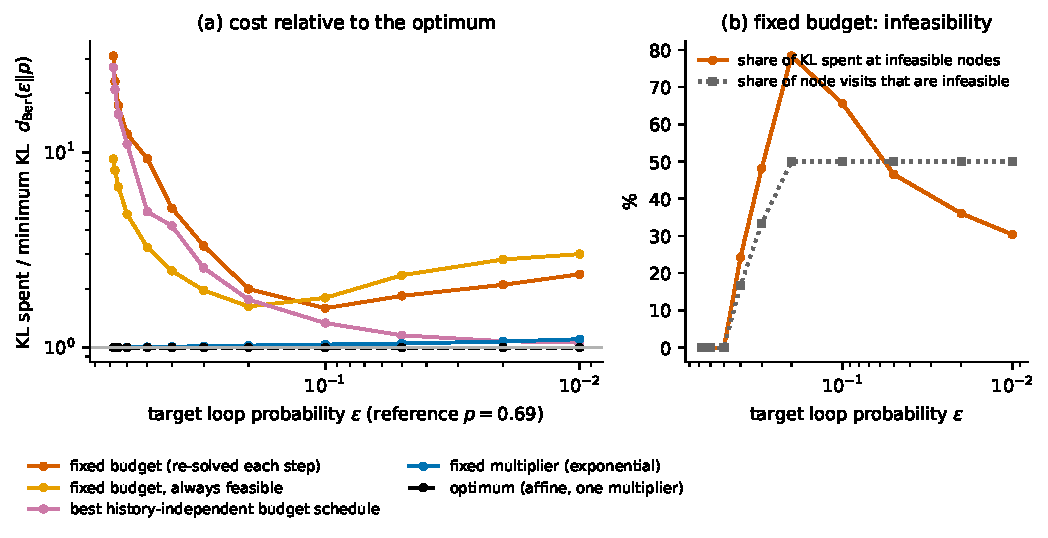
\includegraphics[width=\textwidth]{figures/fig_ladder.pdf}
\caption{Base system. (a) KL spent relative to the minimum KL for the same loop probability, for each rule of the ladder; the fixed price is within 10.3\% of the optimum throughout, the fixed budget is not. (b) Where the fixed-budget controller is infeasible: the share of node visits and the share of its KL spent at infeasible nodes.}\label{fig:ladder}
\end{figure}

\subsection{Infeasibility is not the explanation}\label{ssec:infeas}
A fixed budget is infeasible at a node when it lies below the floor $\min_v H(h,v)$, and Table~\ref{tab:ladder} shows that this affects 17--50\% of node visits at targets $\epsilon\le0.4$. The excess cannot be attributed to this alone, for three reasons.
\begin{enumerate}[leftmargin=*,itemsep=1pt]
\item \emph{The excess exists without any infeasibility.} At $\epsilon\ge0.5$ in the base system no node is infeasible, yet the fixed budget costs 9--31 times the minimum. In the persistent system with $R=3$ and $N=8$ no budget on the grid is infeasible at any target (0\% of node visits), and the fixed budget still costs 2.7--7.1 times the minimum.
\item \emph{Removing infeasibility does not remove the excess.} The always-feasible budget never collapses. It lowers the cost at weak control (12.4$\to$4.8 times at $\epsilon=0.6$) and raises it at strong control (2.4$\to$3.0 times at $\epsilon=0.01$), because with one fixed fraction of headroom at every node it still prices histories very differently ($1+\mathrm{CV}^2\approx11$, Table~\ref{tab:ladder}). Abstaining at infeasible nodes, the other way to avoid them, cannot reach any target below $\epsilon=0.4$ and costs more where it can (6.6 against 5.2 times at $\epsilon=0.4$).
\item \emph{What does remove it is a constant price.} The fixed-price rule has no budget to be infeasible, and its cost is within 12.5\% of the minimum.
\end{enumerate}
Infeasibility is a separate, additional cost that appears at strong control: at $\epsilon=0.2$, 78\% of the fixed-budget controller's KL is spent at nodes where its budget cannot be met. The universal mechanism, present at every target and in every system, is the allocation of distortion across histories.

\subsection{The waste law holds}\label{ssec:lawtest}
\begin{figure}[H]
\centering
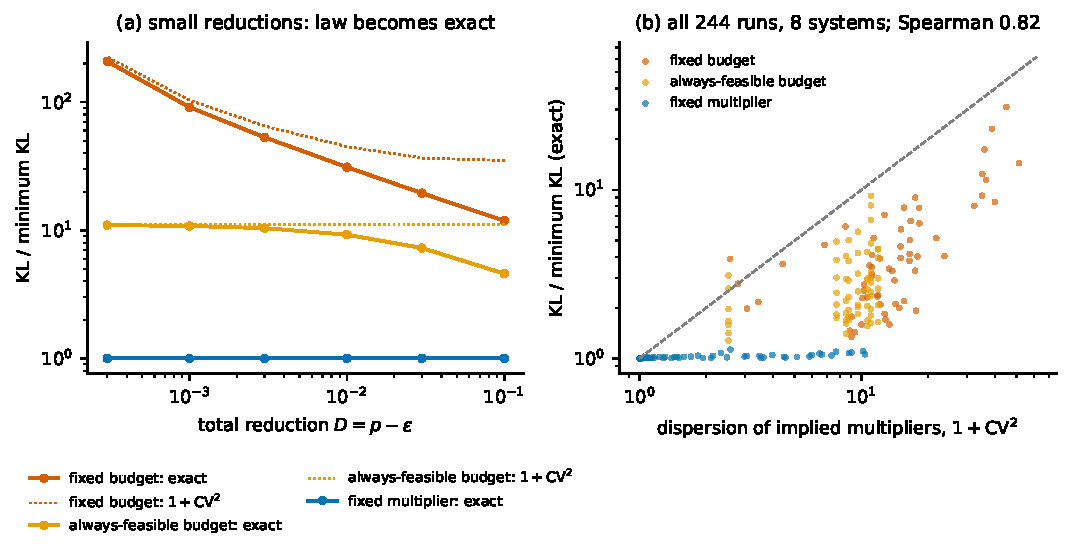
\includegraphics[width=\textwidth]{figures/fig_waste_law.pdf}
\caption{(a) Base system, small reductions $D=p-\epsilon$: the exact cost ratio approaches $1+\mathrm{CV}^2$ for the always-feasible budget (0.994 of the predicted value at $D=3\cdot10^{-4}$) and for the fixed budget (0.93 and rising), while the fixed price stays at 1. The fixed-budget waste grows without bound as $D\to0$. (b) All 244 runs of the eight systems: exact cost ratio against $1+\mathrm{CV}^2$ (Spearman $\rho=0.82$). The law over-predicts when the reduction is large, where the quadratic approximation no longer holds.}\label{fig:waste}
\end{figure}
Proposition~\ref{prop:waste} makes quantitative predictions that the exact computation can test. In the second-order regime the ratio $\KL/d_{\mathrm{Ber}}$ should equal $1+\mathrm{CV}^2$, and for the fixed budget it should be at least $1/\varphi$. Figure~\ref{fig:waste} and Table~\ref{tab:smalld} confirm both: as $D\to0$ the exact ratio converges to $1+\mathrm{CV}^2$, and $1/\varphi$ is a lower bound throughout. Away from the second-order regime the law overstates the waste (it predicts 35 where the exact ratio is 12 at $D=0.1$ for the fixed budget) but orders the controllers correctly: across all 244 runs the rank correlation between $\log(1+\mathrm{CV}^2)$ and the log of the exact ratio is 0.82. The dispersion of the implied prices, not the presence of infeasible steps, is what tracks the waste.

{{TABLE:smalld}}

\subsection{Robustness}
{{TABLE:robust}}
Table~\ref{tab:robust} summarizes the ladder over eight systems. The ordering is the same in each: fixed price $\le$ always-feasible budget $\le$ fixed budget at weak control; the fixed price never exceeds 1.13 times the minimum, and the fixed budget never falls below 1.3. The persistent systems ($R=2,3$), whose events are closer to those of the text experiments, show the same pattern with smaller but still substantial waste (up to 9 times). What the exact systems do not contain is a language model: the hazard here is exact and the state space is small. Section~\ref{sec:real} asks which parts survive.
